\documentclass[aspectratio=169]{beamer}
% \usepackage{amsfonts, amsmath, amssymb, amsthm}
% \usepackage{fancyhdr, float, graphicx}
% \usepackage[utf8]{inputenc} % Required for inputting international characters
% \usepackage[T1]{fontenc} % Output font encoding for international characters
% \usepackage{fouriernc} % Use the New Century Schoolbook font
% \usepackage[nottoc, notlot, notlof]{tocbibind}
% \usepackage{listings}
% \usepackage{xcolor}
% \usepackage{blindtext}
\usepackage{verbatim}
\usepackage{multicol}
% \usepackage{hyperref}
% Theme
% good themes are Singapore, CambridgeUS, Boadilla or none
\usetheme{}
% good color themes are seahorse, crane, beaver, dolphin, lily
\usecolortheme{beaver}

\renewcommand{\familydefault}{\rmdefault}

% Title page
\title{Machine Learning Powered Automated Facial Attendanc Tracking System}
\author{Mid Term Status and Progress Evaluation}
\date{\today}

\begin{document}

\begin{frame}
	\titlepage
\end{frame}

\begin{frame}
	\frametitle{Content}
	\tableofcontents
\end{frame}

\section{Status Overview}

\begin{frame}
	\centering
	\frametitle{Status Overview}
	\begin{minipage}{0.95\textwidth}
		\textbf{Frontend}
		\begin{enumerate}
			\item App Implementation is 50 \% complete.
			\item Integration with Backend is pending.
		\end{enumerate}
		\textbf{Backend}
		\begin{enumerate}
			\item Backend Implementation of APIs is 80 \% complete.
			\item Core functions are working.
			\item Integration with Frontend is pending.
			\item Improvement in Face Recognition is pending.
		\end{enumerate}
	\end{minipage}
\end{frame}


\section{Frontend Technologies}
\begin{frame}
	\centering
	\frametitle{Frontend Technologies}
	\begin{minipage}{0.95\textwidth}
		\textbf{Libraries Used for Creating Cross Platform App}
		\begin{enumerate}
			\item React Native
			\item Axios
			\item React Navigation
		\end{enumerate}
	\end{minipage}
\end{frame}


\begin{frame}
	\centering
	\frametitle{React Native}
	\framesubtitle{Overview and Features}
	\begin{minipage}{0.95\textwidth}
		\textbf{React Native}
		\begin{enumerate}
			\item React Native is a JavaScript framework for writing real, natively rendering mobile applications for iOS and Android.
			\item It’s based on React, Facebook’s JavaScript library for building user interfaces, but instead of targeting the browser, it targets mobile platforms.
			\item Its Cross Platform, meaning it will work on both iOS and Android, \textit{which are the primary Operating systems our teachers use.}
		\end{enumerate}
	\end{minipage}
\end{frame}


\begin{frame}
	\centering
	\frametitle{React Native}
	\framesubtitle{Cross Platform App Development}
	\begin{minipage}{0.95\textwidth}
		\begin{figure}[H]
			\centering
			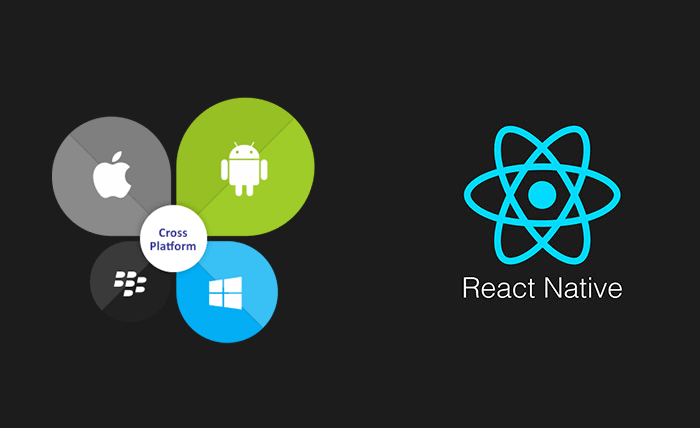
\includegraphics[width=.85\textwidth]{react native 2.png}
		\end{figure}
	\end{minipage}
\end{frame}



\section{Frontend Drafts}
\begin{frame}
	\centering
	\frametitle{Frontend Drafts}
	\framesubtitle{These are the initial drafts of the app}
	\begin{figure}[H]
		\centering
		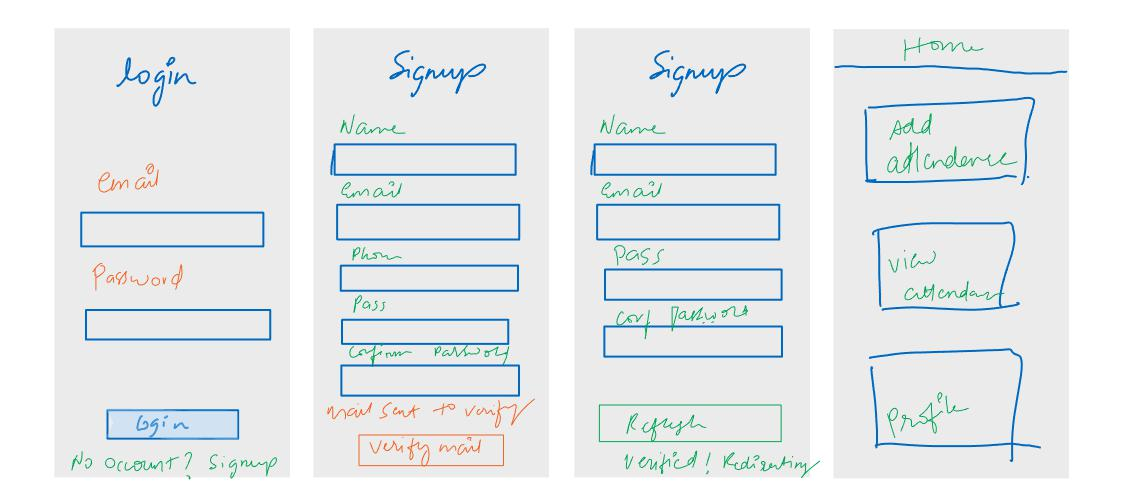
\includegraphics[width=.95\textwidth]{../../Diagrams/first 4.jpg}
		\caption{Drafts of the App}
	\end{figure}
\end{frame}


\begin{frame}
	\centering
	\frametitle{Frontend Progress}
	\framesubtitle{Current Progress in App Development (Mid Term Stage)}
	\begin{figure}[H]
		\centering
		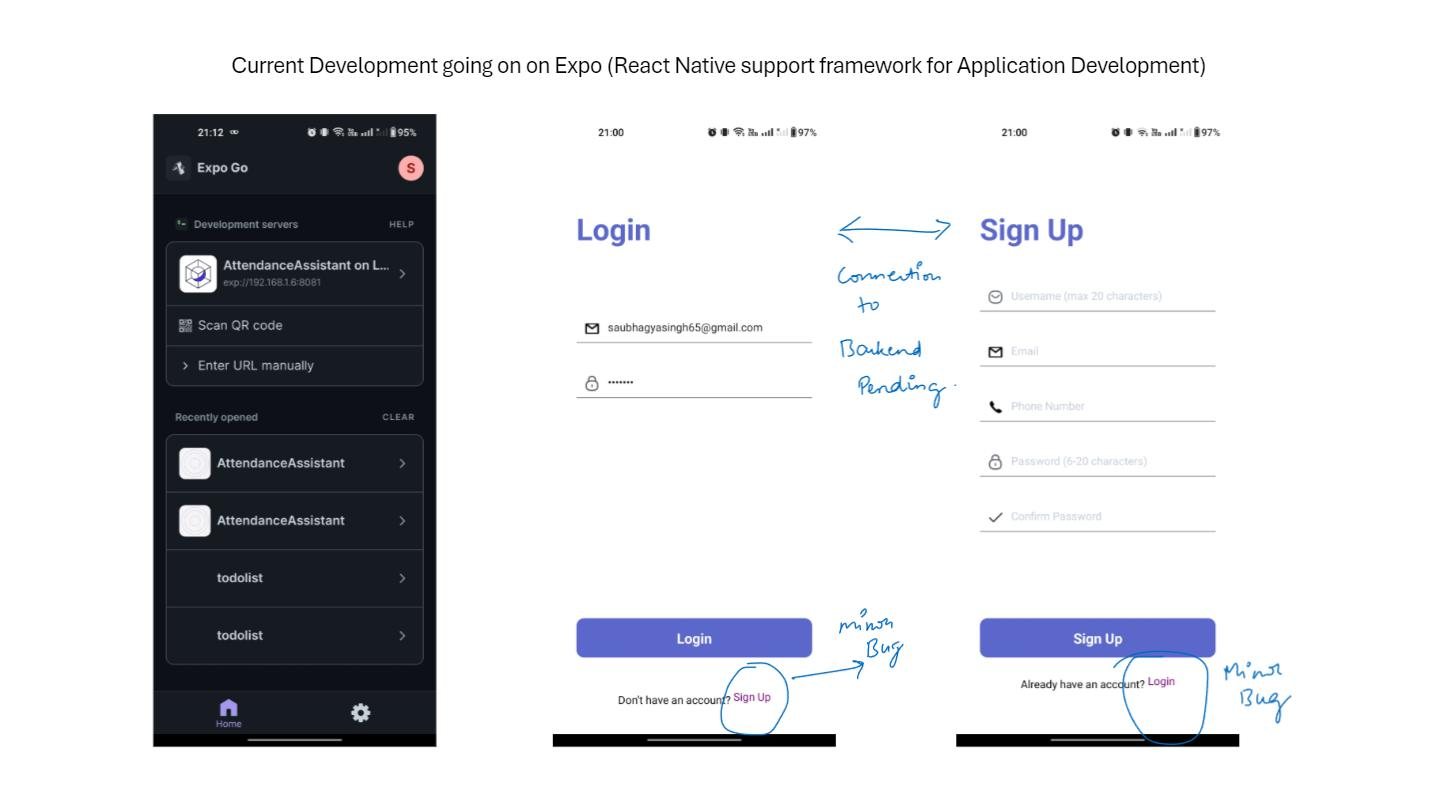
\includegraphics[width=.99\textwidth]{../../Frontend Status/Mid Term/frontend app status for mini proj eval.jpg}
	\end{figure}
\end{frame}

\begin{frame}
	\centering
	\frametitle{Frontend Progress}
	\framesubtitle{Current Progress in App Development (Mid Term Stage) Continued}
	\begin{figure}[H]
		\centering
		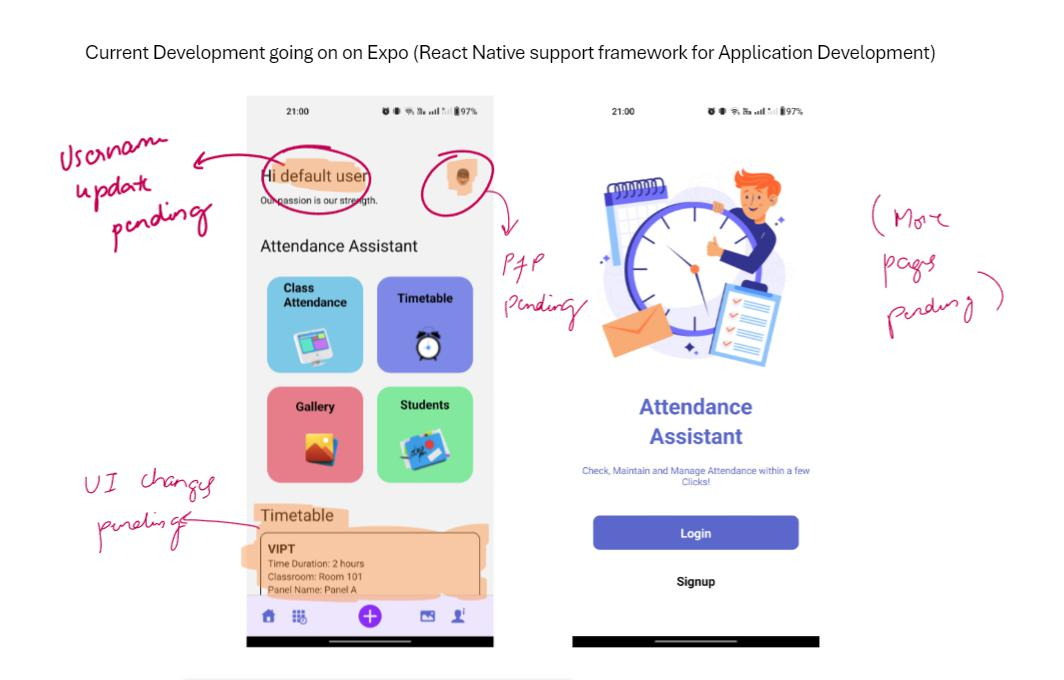
\includegraphics[width=.8\textwidth]{../../Frontend Status/Mid Term/frontend app status for mini proj 2.jpg}
	\end{figure}
\end{frame}

\section{Frontend Work Remaining}
\begin{frame}
	\centering
	\frametitle{Frontend Work Remaining}
	\begin{minipage}{0.95\textwidth}
		\begin{enumerate}
			\item Integration with Backend.
			\item Improving User Interface.
			\item Adding Core Features of taking photos and uploading Attendance
		\end{enumerate}
	\end{minipage}
\end{frame}

\section{Backend Technologies}
\begin{frame}
	\centering
	\frametitle{Backend Technologies}
	\begin{minipage}{0.95\textwidth}
		\begin{enumerate}
			\item FastAPI for creating APIs.
			\item MongoDB for Database.
			\item Multiple Face Recognition Libraries
			\item Python for Backend Development
			\item Docker for Containerization
			\item Swagger for API Documentation
		\end{enumerate}
	\end{minipage}
\end{frame}

\begin{frame}
	\centering
	\frametitle{FastAPI}
	\framesubtitle{Overview}
	\begin{minipage}{0.95\textwidth}
		\begin{enumerate}
			\item FastAPI is a modern, fast (high-performance), web framework for building APIs with Python 3.6+ based on standard Python type hints.
			\item It is based on standard Python type hints, which makes it easy to use and understand.
			\item It is one of the fastest Python frameworks available.
		\end{enumerate}
	\end{minipage}
\end{frame}

\begin{frame}
	\centering
	\frametitle{FastAPI}
	\framesubtitle{In Use}
	\begin{figure}[H]
		\centering
		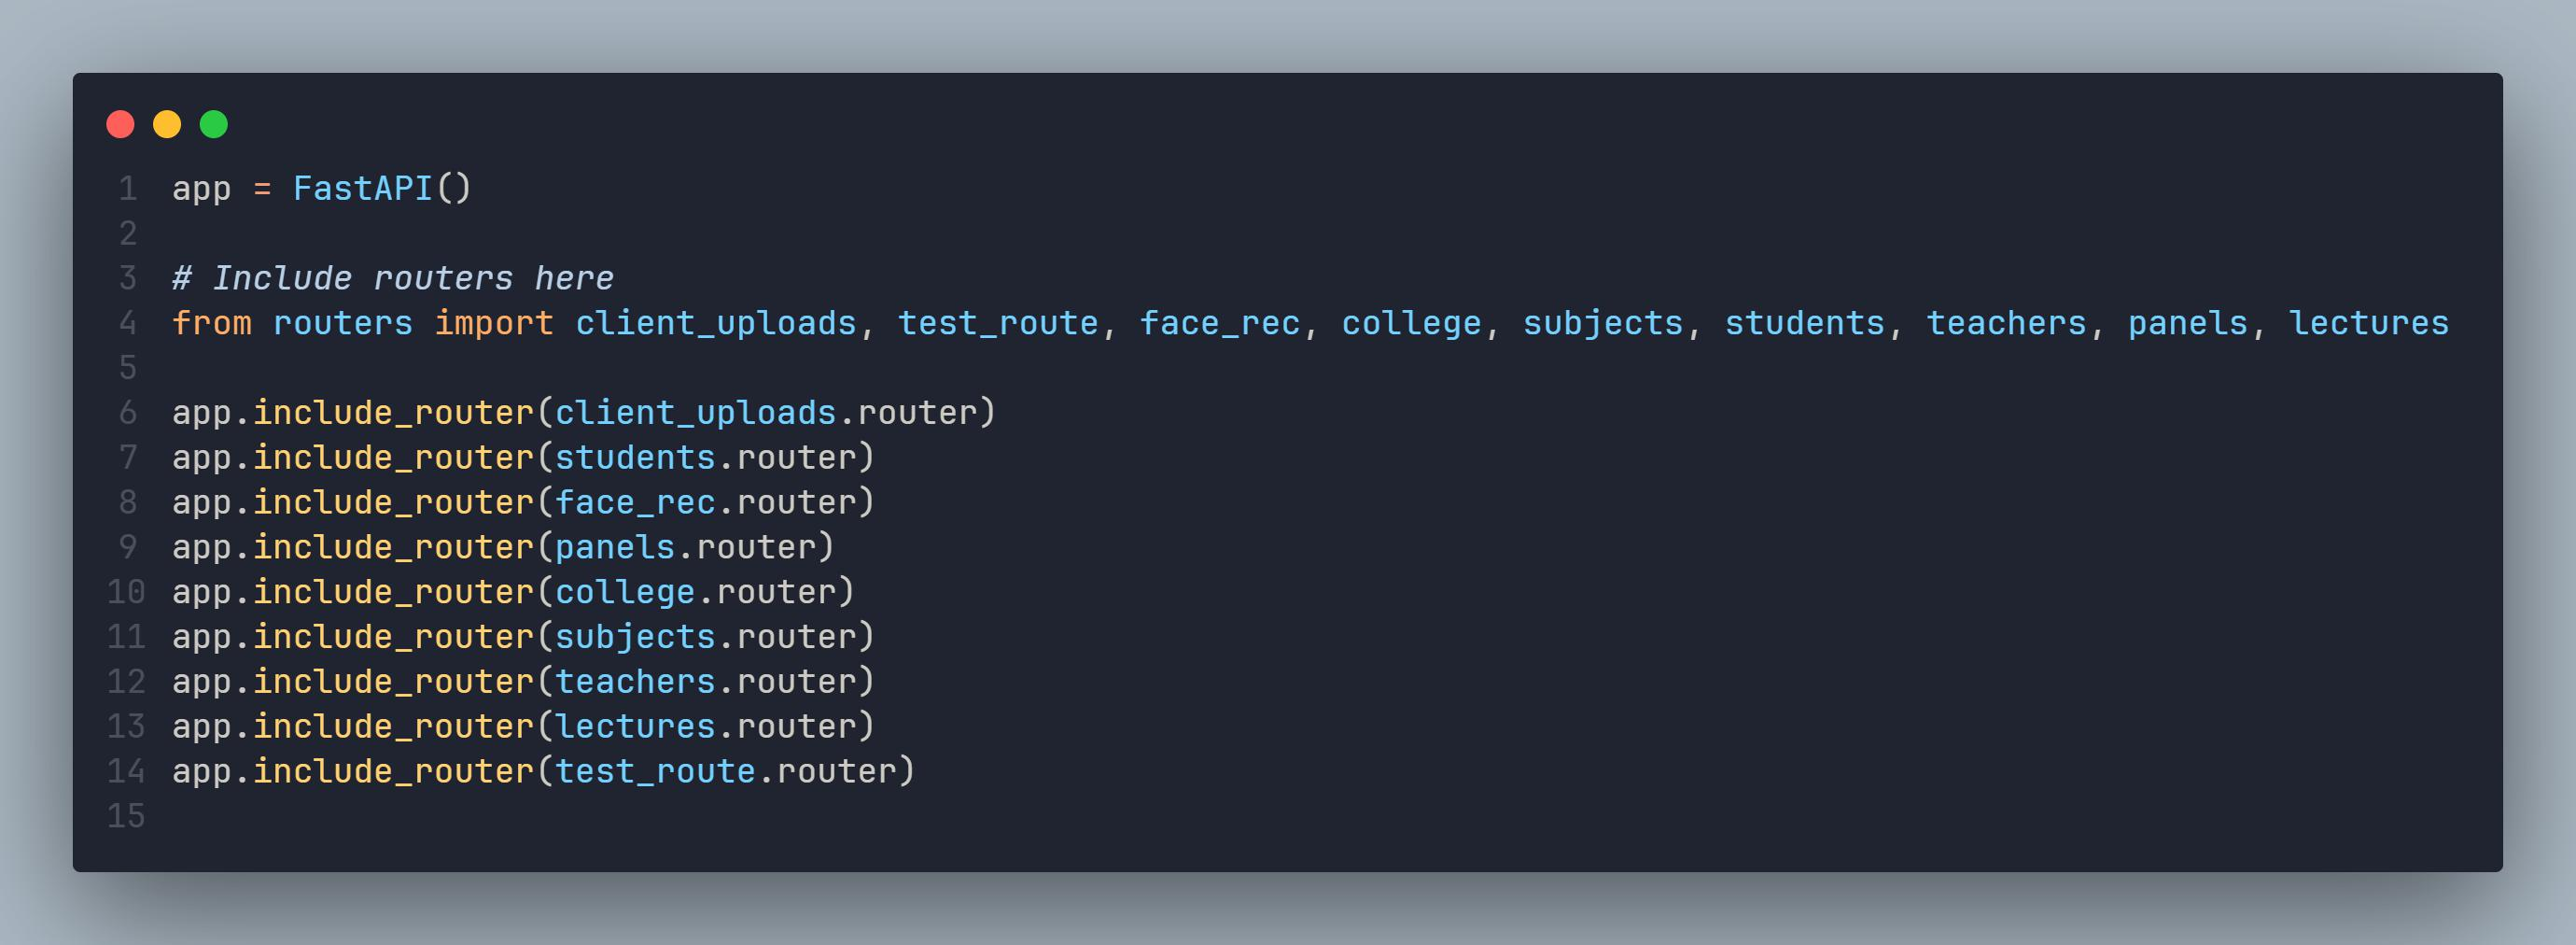
\includegraphics[width=.95\textwidth]{fastapi.jpg}
	\end{figure}
\end{frame}

\begin{frame}
	\centering
	\frametitle{Swagger for API Documentation}
	\framesubtitle{Overview}
	\begin{minipage}{0.95\textwidth}
		\begin{enumerate}
			\item Swagger is a set of open-source tools built around the OpenAPI Specification that can help you design, build, document and consume REST APIs.
			\item It is used to document the APIs in a user friendly way.
			\item It is used to test the APIs.
			\item It is used to generate client libraries for the APIs.
			\item It is used to generate server stubs for the APIs.
			\item It is default with FastAPI.
		\end{enumerate}
	\end{minipage}
\end{frame}

\begin{frame}
	\centering
	\frametitle{MongoDB for Database}
	\framesubtitle{Overview}
	\begin{minipage}{0.95\textwidth}
		\begin{enumerate}
			\item MongoDB is a general purpose, document-based, distributed database built for modern application developers and for the cloud era.
			\item It is a NoSQL database, which means it stores data in JSON-like documents.
			\item It is used to store the data of the students and their faces.
		\end{enumerate}
	\end{minipage}
\end{frame}
\begin{frame}
	\centering
	\frametitle{MongoDB for Database}
	\framesubtitle{In Use}
	\begin{minipage}{0.95\textwidth}
		\begin{figure}[H]
			\centering
			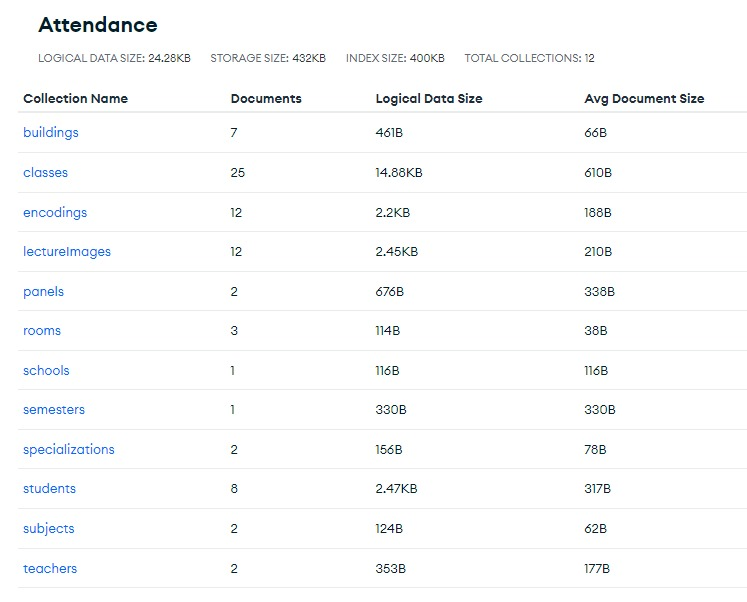
\includegraphics[width=.85\textwidth]{mongo.jpg}
		\end{figure}
	\end{minipage}
\end{frame}


\section{Backend Drafts}
\begin{frame}
	\centering
	\frametitle{Backend Drafts}
	\begin{minipage}{0.95\textwidth}
		the readme file from github etc
	\end{minipage}
\end{frame}
\section{Backend Work Done}
\begin{frame}
	\centering
	\frametitle{Backend Work Done}
	\begin{minipage}{0.95\textwidth}
		\begin{enumerate}
			\item Core APIs are working.
			\item Face Recognition is working.
			\item Database is working.
			\item Swagger Documentation is complete.
			\item Docker Containerization is complete.
		\end{enumerate}
	\end{minipage}
\end{frame}

\begin{frame}
	\centering
	\frametitle{API}
	\framesubtitle{Uploading Images from App or Pi or Website}
	\begin{minipage}{0.95\textwidth}
		\begin{figure}[H]
			\centering
			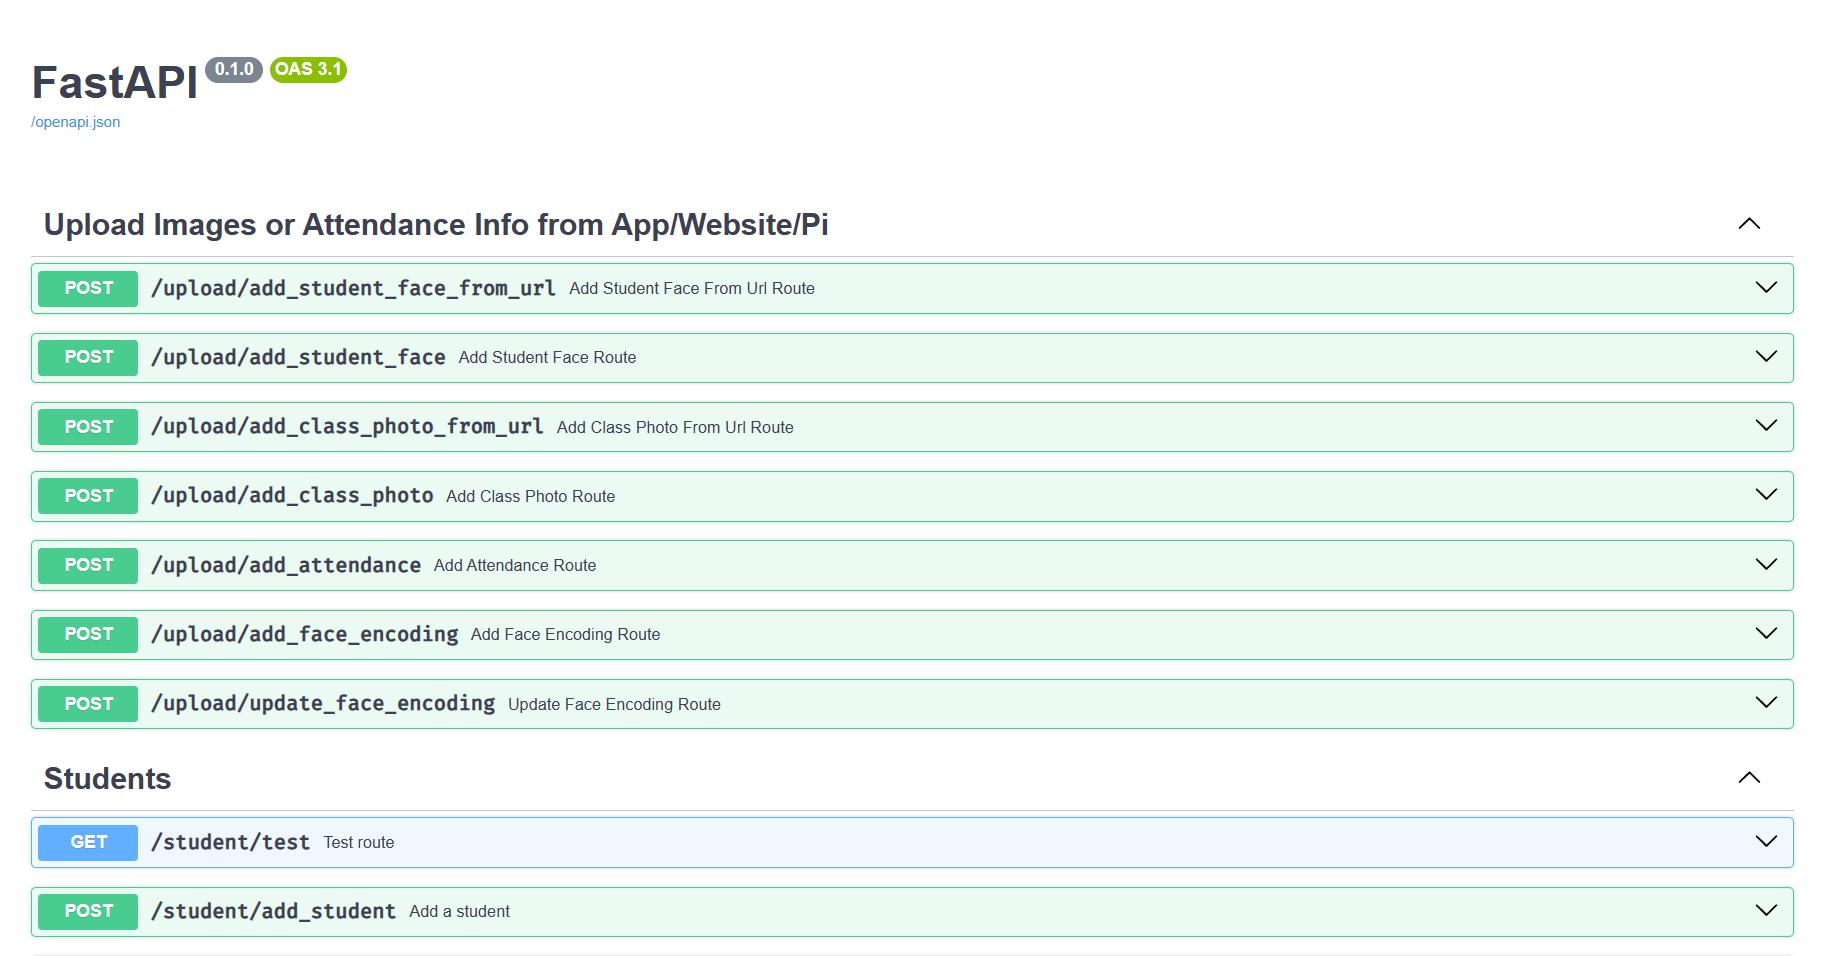
\includegraphics[width=.95\textwidth]{swagger 1.jpg}
		\end{figure}
	\end{minipage}
\end{frame}

\begin{frame}
	\centering
	\frametitle{API}
	\framesubtitle{The Model to add attendance (from Teachers App only)}
	\begin{minipage}{0.95\textwidth}
		\begin{figure}[H]
			\centering
			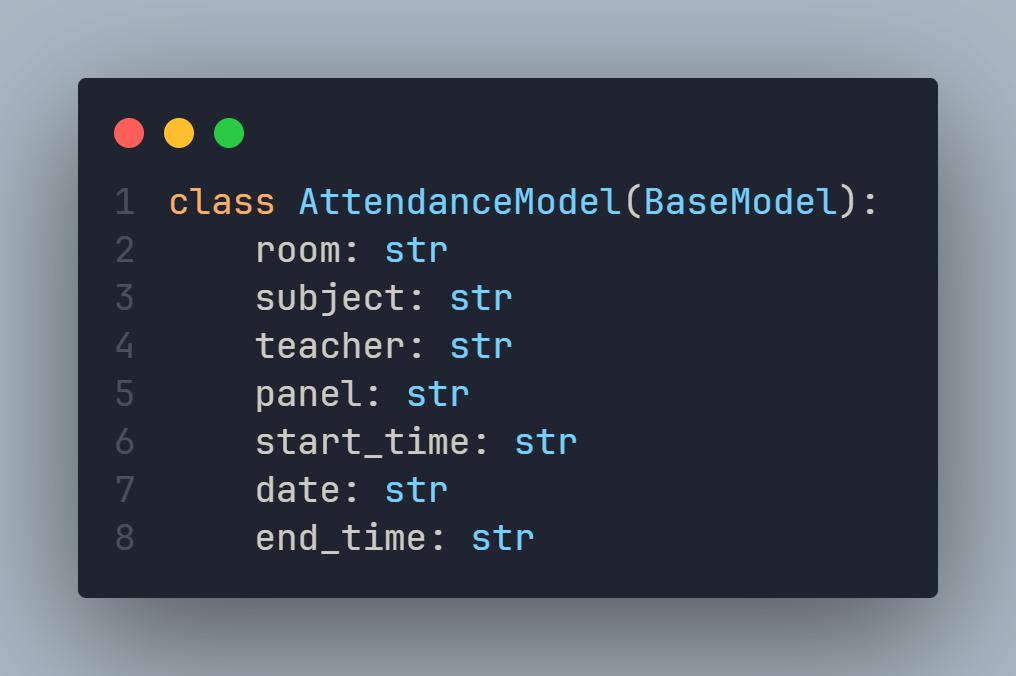
\includegraphics[width=.65\textwidth]{Clipboard Image.jpg}
		\end{figure}
	\end{minipage}
\end{frame}
\begin{frame}
	\centering
	\frametitle{API}
	\framesubtitle{Students API}
	\begin{minipage}{0.95\textwidth}
		\begin{figure}[H]
			\centering
			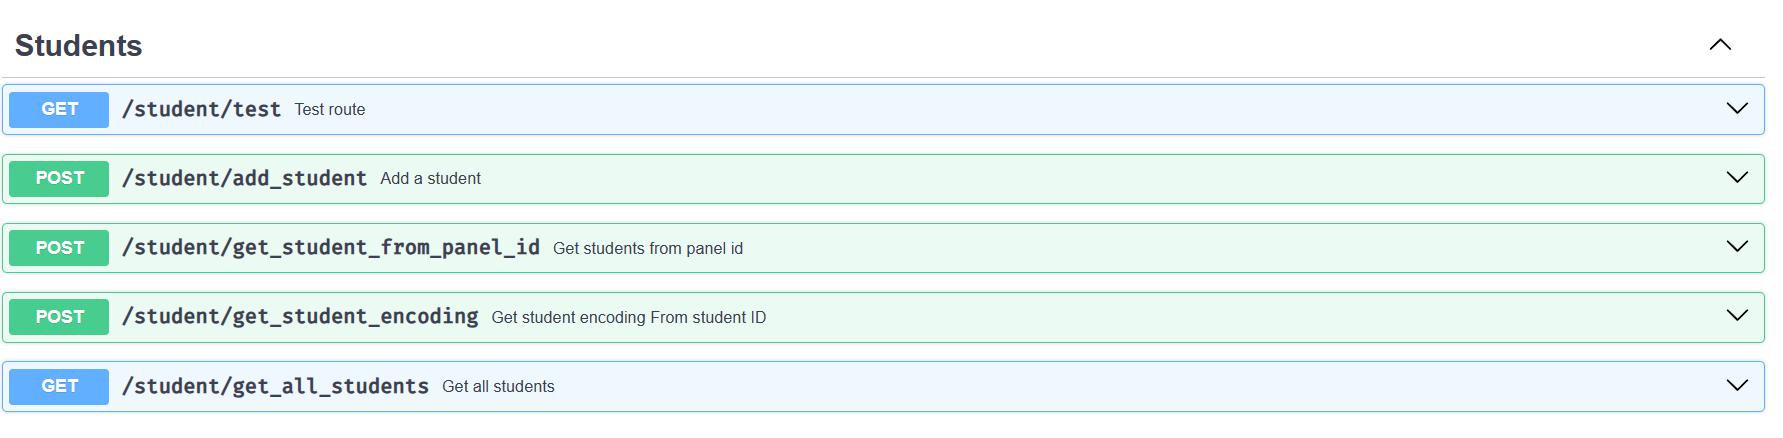
\includegraphics[width=.95\textwidth]{swagger 2.jpg}
		\end{figure}
	\end{minipage}
\end{frame}
\begin{frame}
	\centering
	\frametitle{API}
	\framesubtitle{Students Models}
	\begin{minipage}{0.95\textwidth}
		\begin{figure}[H]
			\centering
			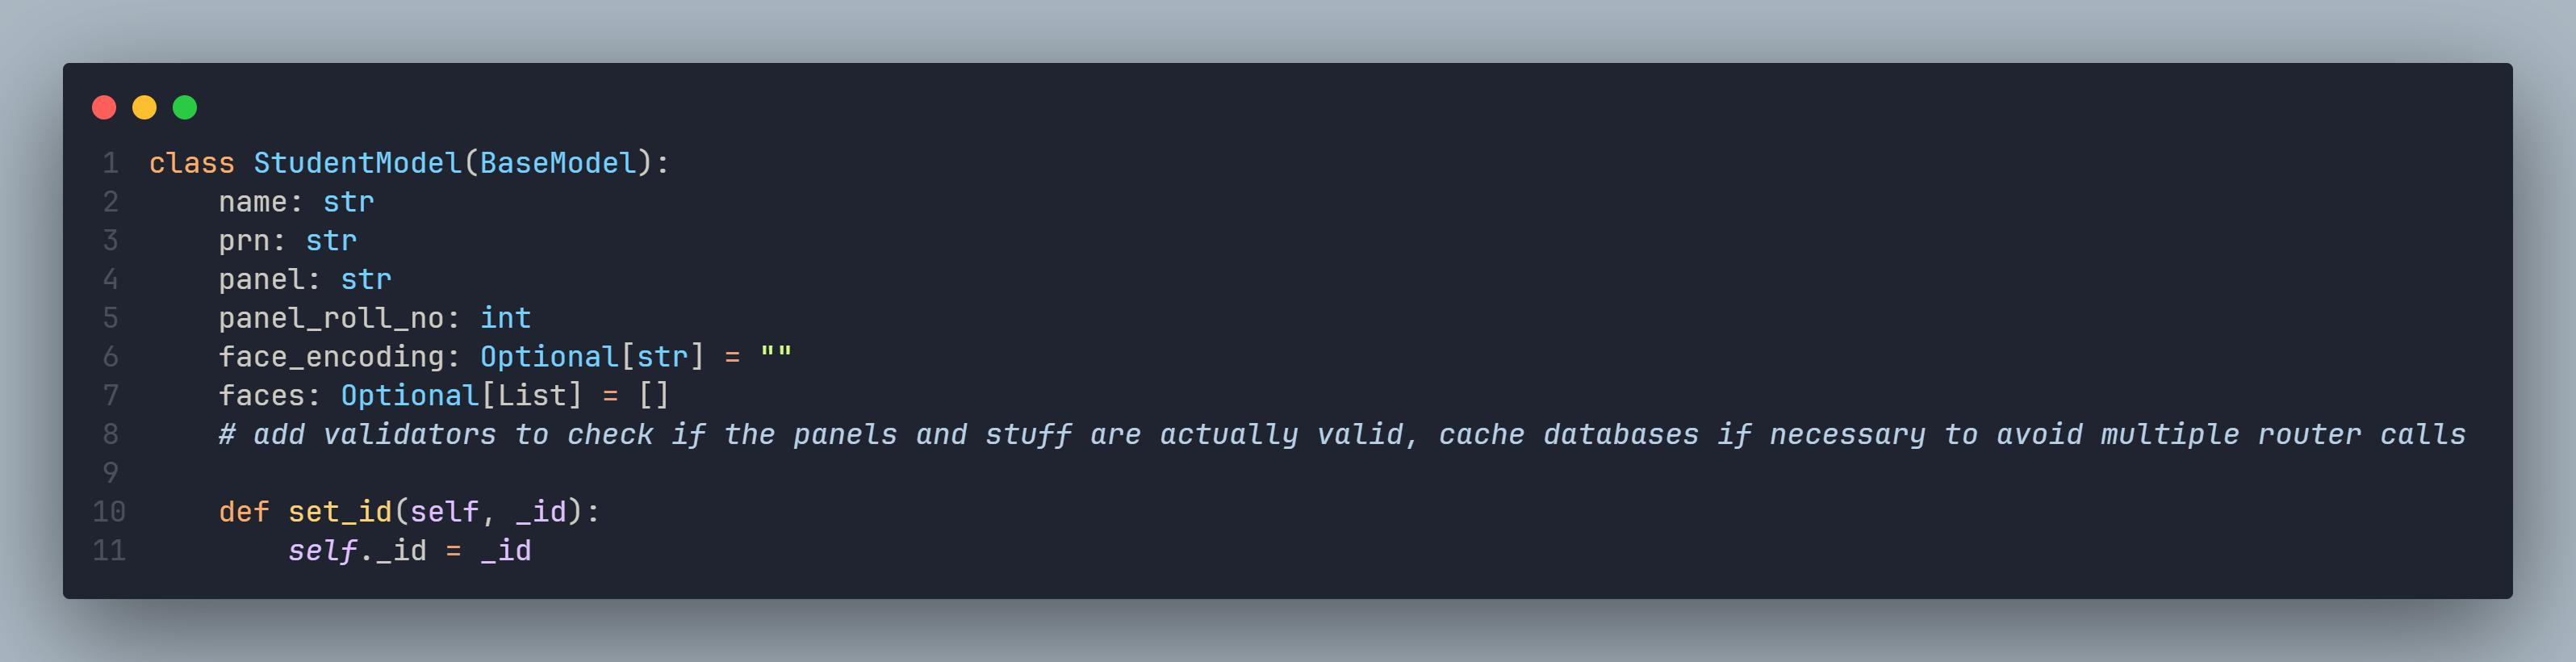
\includegraphics[width=.99\textwidth]{student.jpg}
		\end{figure}
	\end{minipage}
\end{frame}


\begin{frame}
	\centering
	\frametitle{API}
	\framesubtitle{Face Recognition and Panels}
	\begin{minipage}{0.95\textwidth}
		\begin{figure}[H]
			\centering
			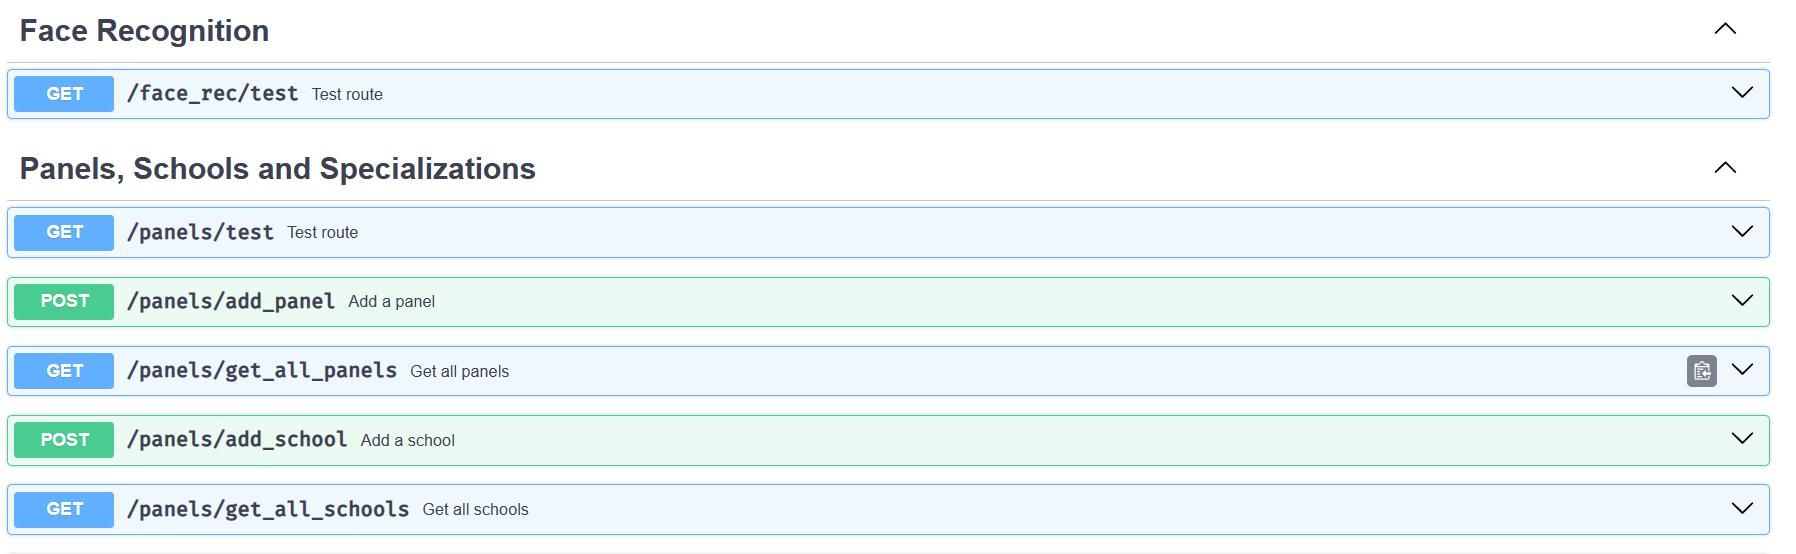
\includegraphics[width=.95\textwidth]{swagger 3.jpg}
		\end{figure}
	\end{minipage}
\end{frame}
\begin{frame}
	\centering
	\frametitle{API}
	\framesubtitle{Panels Continued}
	\begin{minipage}{0.95\textwidth}
		\begin{figure}[H]
			\centering
			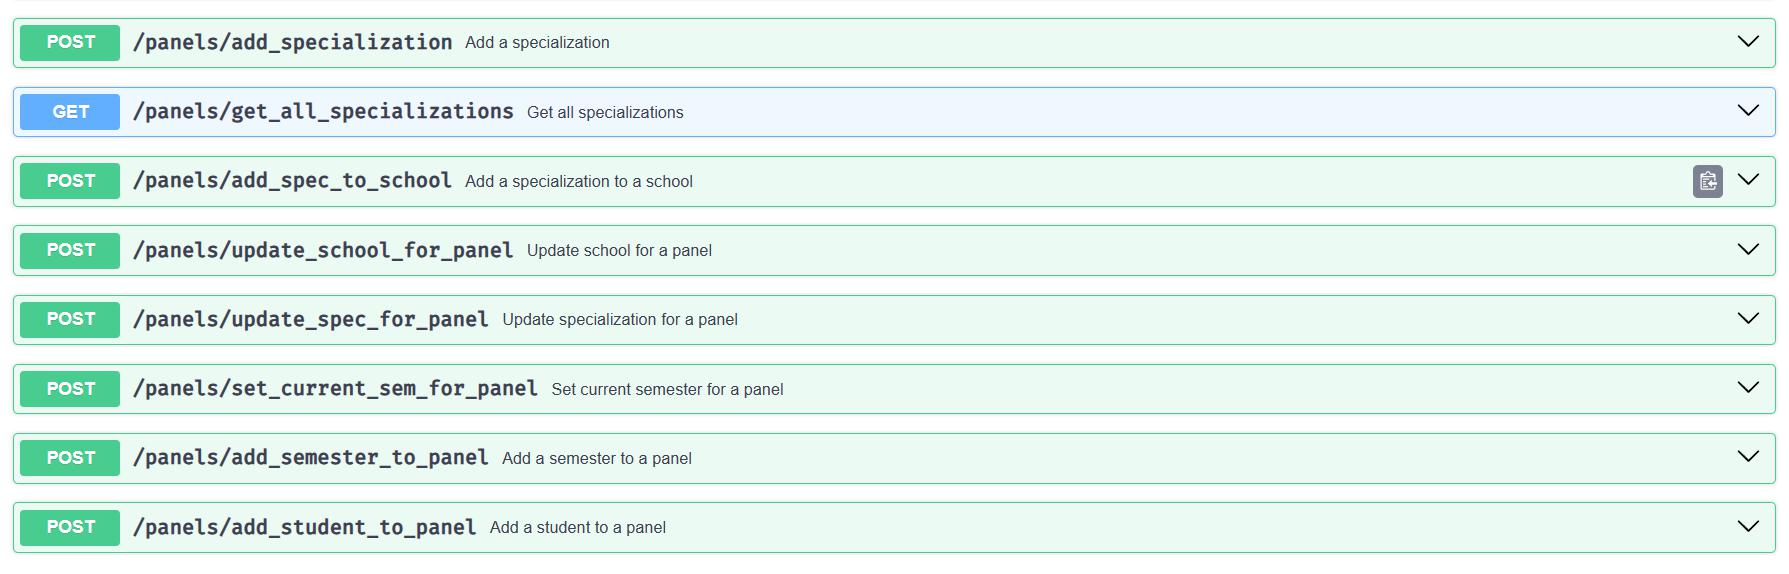
\includegraphics[width=.95\textwidth]{swagger 4.jpg}
		\end{figure}
	\end{minipage}
\end{frame}
\begin{frame}
	\centering
	\frametitle{API}
	\framesubtitle{Panel Models}
	\begin{minipage}{0.95\textwidth}
		\begin{figure}[H]
			\centering
			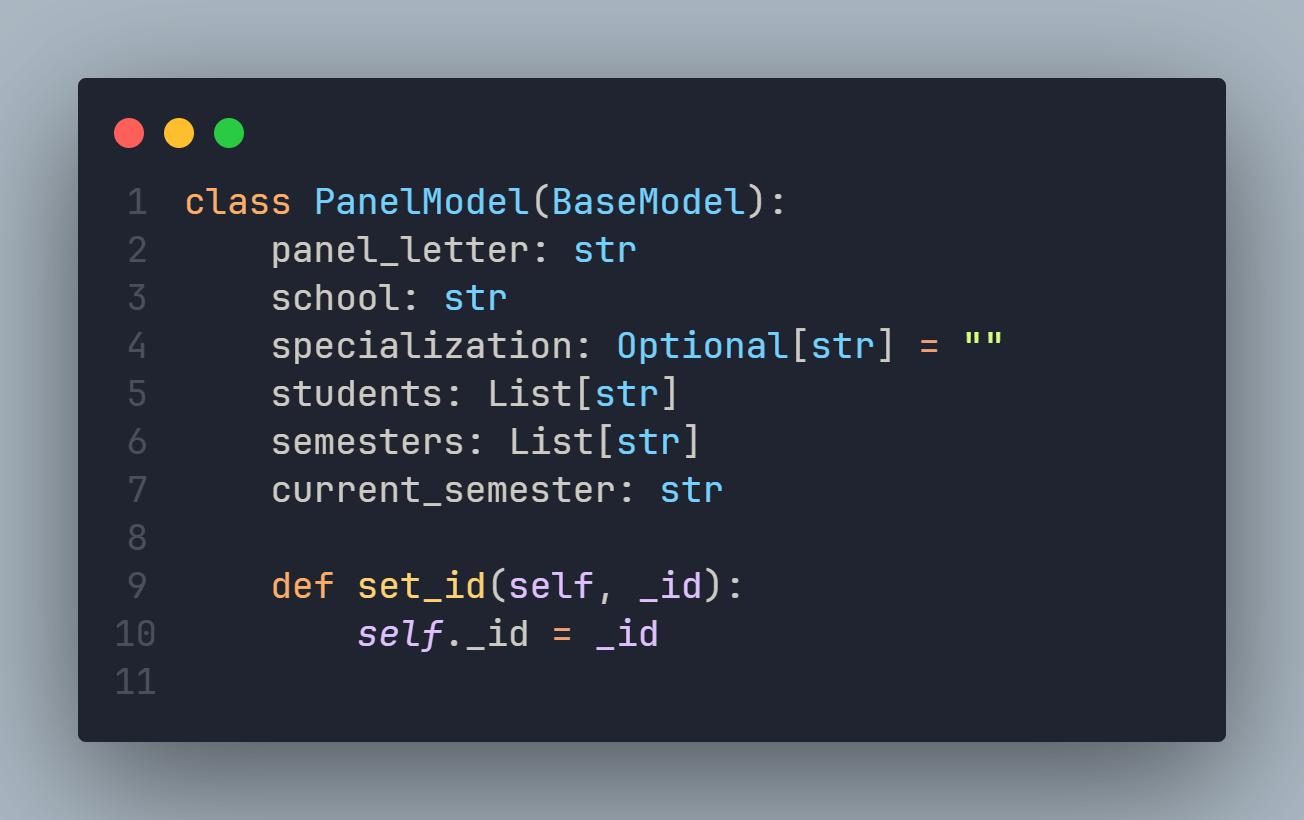
\includegraphics[width=.65\textwidth]{panel.jpg}
		\end{figure}
	\end{minipage}
\end{frame}



\begin{frame}
	\centering
	\frametitle{API}
	\framesubtitle{Rooms and Buildings}
	\begin{minipage}{0.95\textwidth}
		\begin{figure}[H]
			\centering
			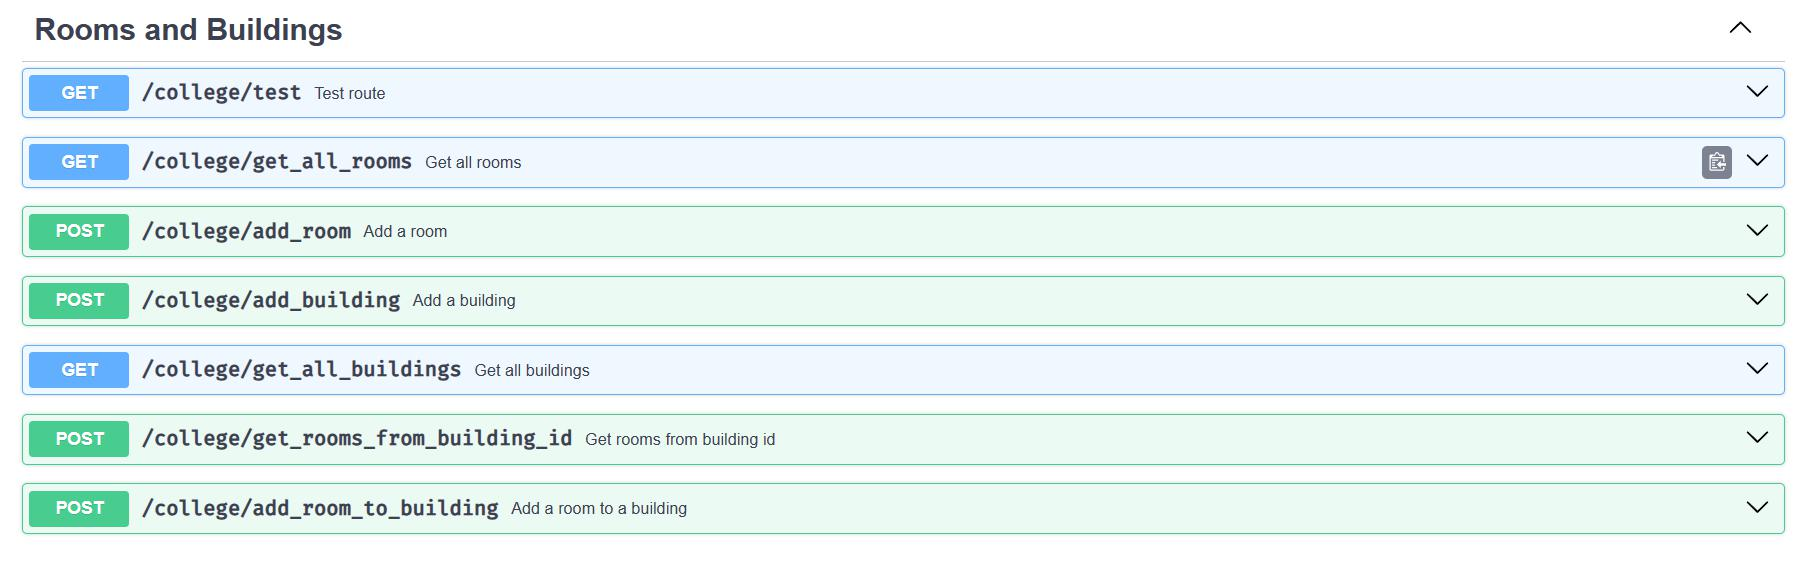
\includegraphics[width=.95\textwidth]{swagger 5.jpg}
		\end{figure}
	\end{minipage}
\end{frame}


\begin{frame}
	\centering
	\frametitle{API}
	\framesubtitle{Models to Manage Rooms and Buildings}
	\begin{minipage}{0.95\textwidth}
		\begin{figure}[H]
			\centering
			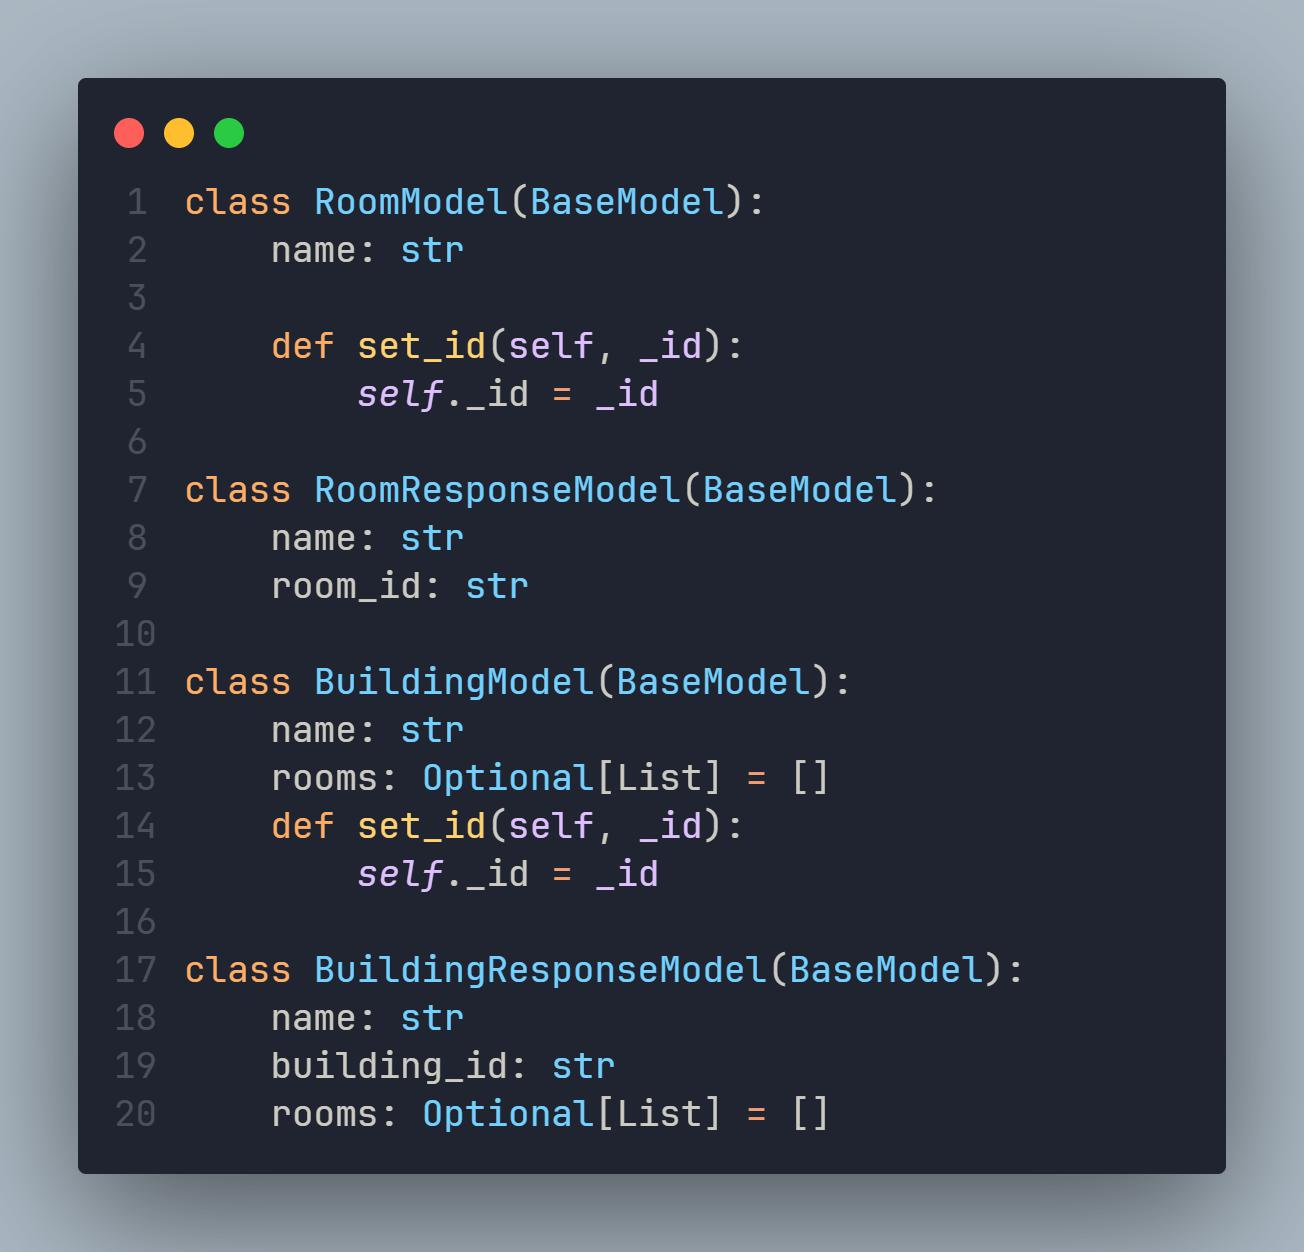
\includegraphics[width=.55\textwidth]{college.jpg}
		\end{figure}
	\end{minipage}
\end{frame}


\begin{frame}
	\centering
	\frametitle{API}
	\framesubtitle{Subjects and Semester}
	\begin{minipage}{0.95\textwidth}
		\begin{figure}[H]
			\centering
			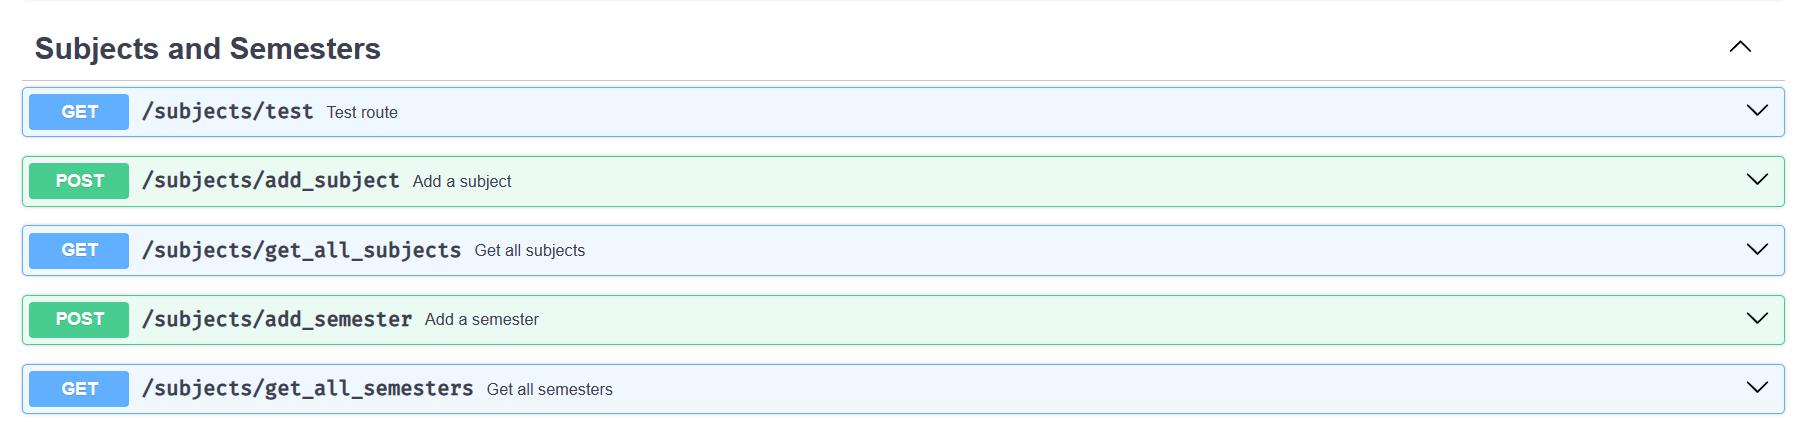
\includegraphics[width=.95\textwidth]{swagger 6.jpg}
		\end{figure}
	\end{minipage}
\end{frame}

\begin{frame}
	\centering
	\frametitle{API}
	\framesubtitle{Semester Model to be added from Admin Page}
	\begin{minipage}{0.95\textwidth}
		\begin{figure}[H]
			\centering
			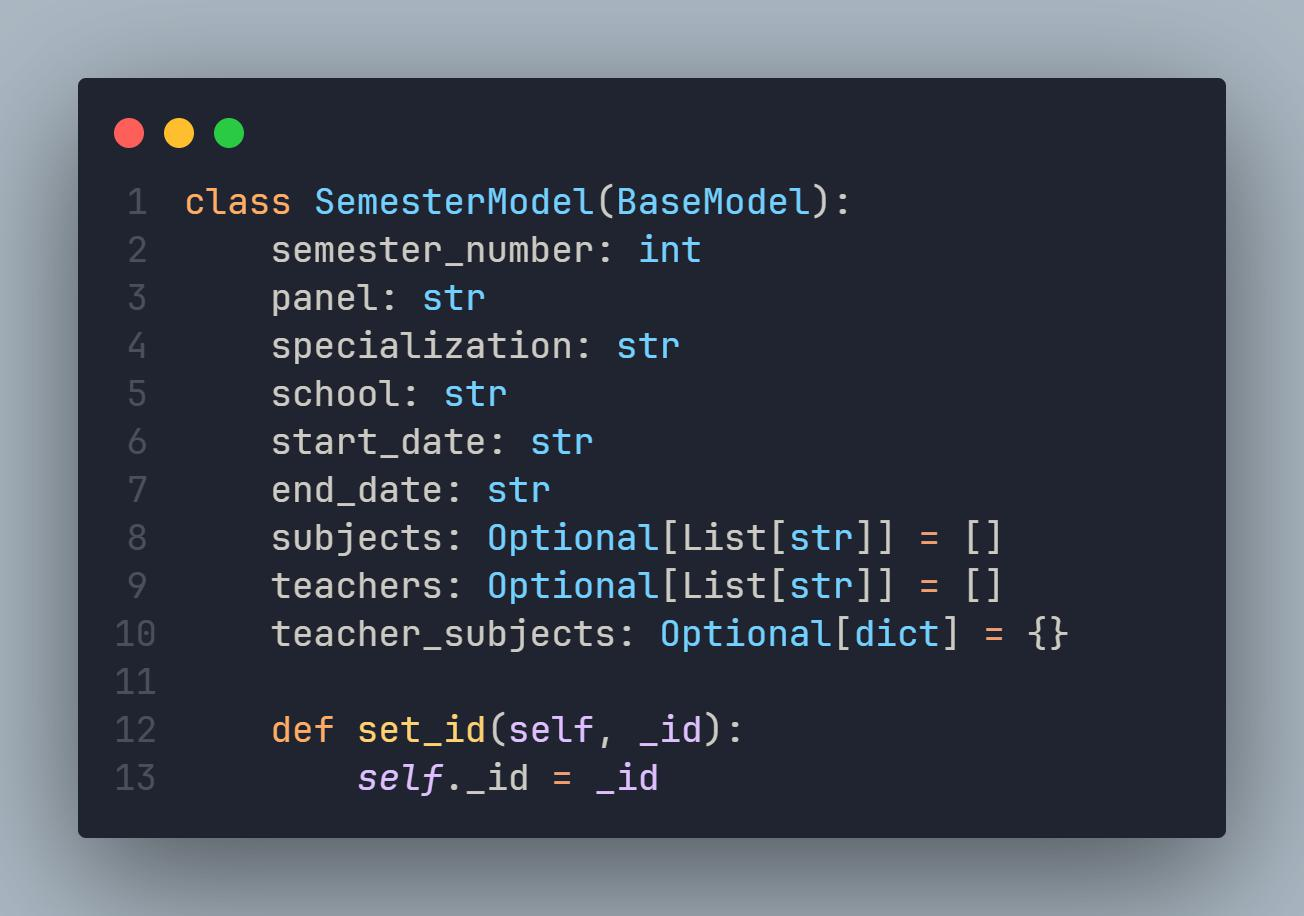
\includegraphics[width=.65\textwidth]{semester.jpg}
		\end{figure}
	\end{minipage}
\end{frame}

\begin{frame}
	\centering
	\frametitle{API Documentation}
	\framesubtitle{Teachers API, used during Signup}
	\begin{minipage}{0.95\textwidth}
		\begin{figure}[H]
			\centering
			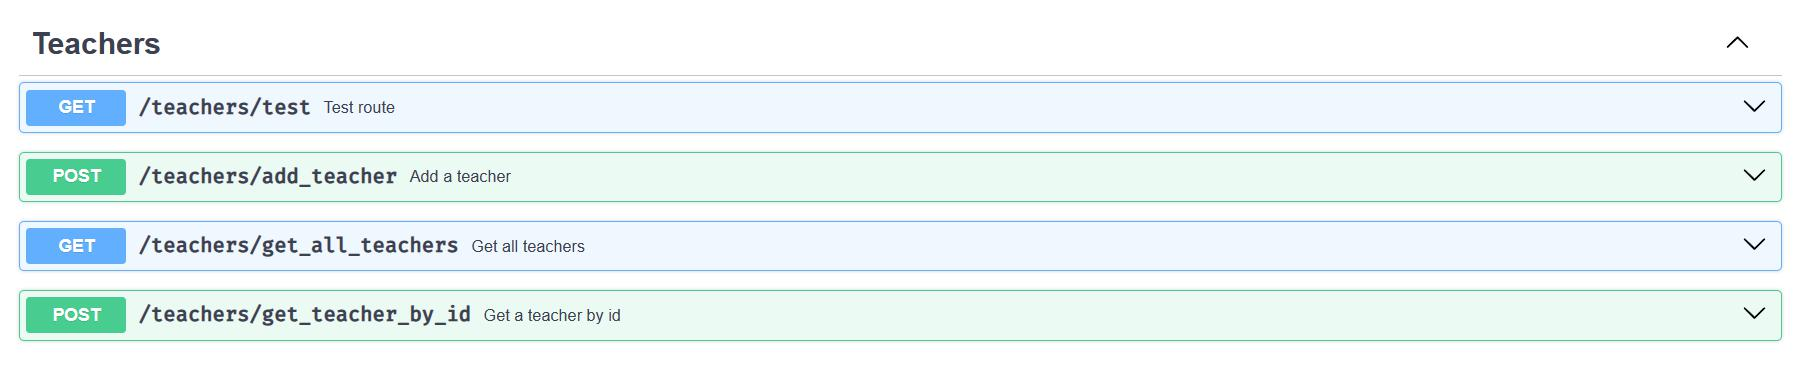
\includegraphics[width=.95\textwidth]{swagger 7.jpg}
		\end{figure}
	\end{minipage}
\end{frame}


\begin{frame}
	\centering
	\frametitle{API}
	\framesubtitle{Teacher Model}
	\begin{minipage}{0.95\textwidth}
		\begin{figure}[H]
			\centering
			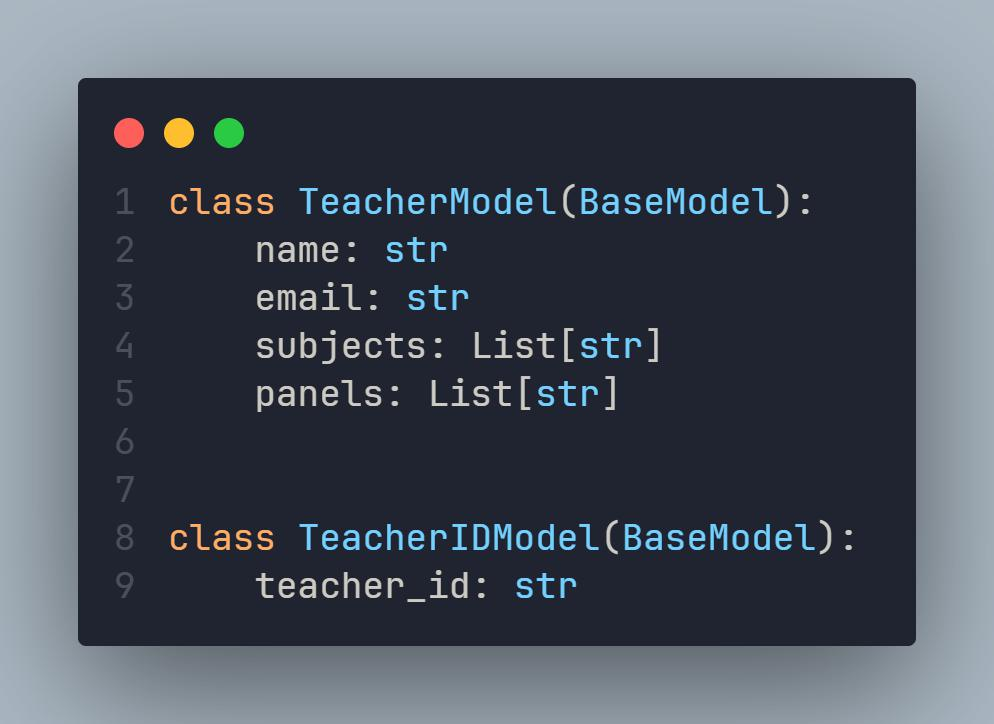
\includegraphics[width=.75\textwidth]{teacher.jpg}
		\end{figure}
	\end{minipage}
\end{frame}

\begin{frame}
	\centering
	\frametitle{API}
	\framesubtitle{Lecture API, used when adding Attendance}
	\begin{minipage}{0.95\textwidth}
		\begin{figure}[H]
			\centering
			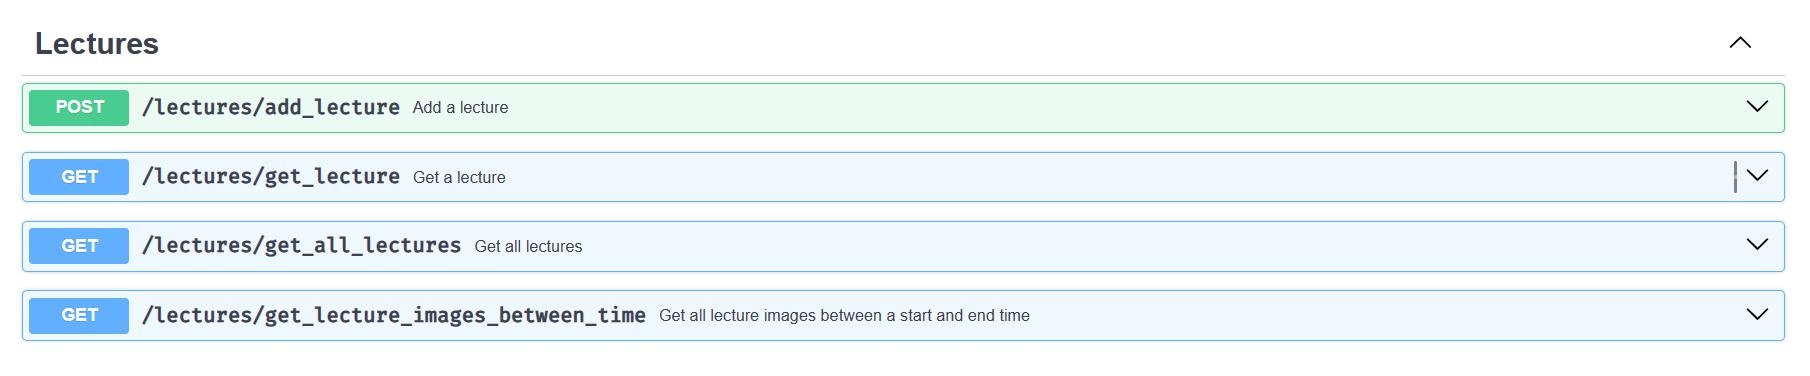
\includegraphics[width=.95\textwidth]{swagger 8.jpg}
		\end{figure}
	\end{minipage}
\end{frame}
\begin{frame}
	\centering
	\frametitle{API}
	\framesubtitle{Lecture Models}
	\begin{minipage}{0.95\textwidth}
		\begin{figure}[H]
			\centering
			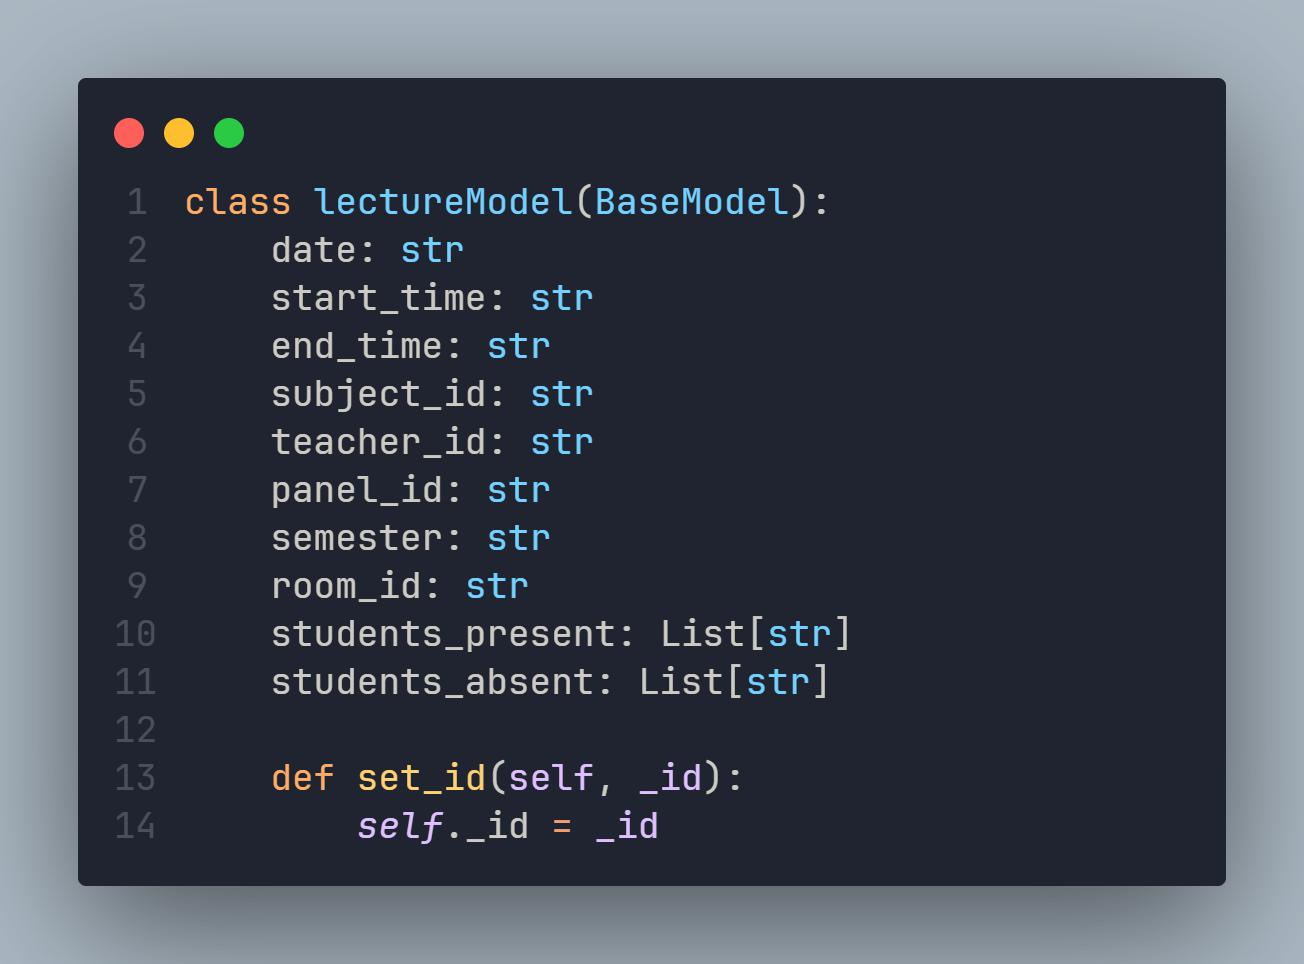
\includegraphics[width=.65\textwidth]{lecture.jpg}
		\end{figure}
	\end{minipage}
\end{frame}

\section{Face Recognition Libraries Used}
\begin{frame}
	\centering
	\frametitle{Face Recognition Libraries Used}
	\framesubtitle{These are the libraries on which all images will be trained and tested. }
	\begin{minipage}{0.95\textwidth}
		\begin{enumerate}
			\item \textcolor{blue}{\textbf{\textit{face\_recognition}}}: A simple face recognition library for Python. It is used to recognize the faces in the images, and to compare the faces.
			\item \textbf{\textit{OpenCV}}: Open Source Computer Vision Library. It is used to detect the faces in the images.
			\item \textbf{\textit{dlib}}: A toolkit for making real world machine learning and data analysis applications in C++. It is used to detect the faces in the images.
			\item \textbf{\textit{DeepFace}}: A lightweight face recognition and facial attribute analysis
		\end{enumerate}
	\end{minipage}
	\footnote{Marked in blue have been used so far. }
\end{frame}
\begin{frame}
	\centering
	\frametitle{Face Recognition Libraries To Use}
	\framesubtitle{Continued}
	\begin{minipage}{0.95\textwidth}
		\begin{enumerate}
			\item \textbf{\textit{imutils}}: A series of convenience functions to make basic image processing functions such as translation, rotation, resizing, skeletonization, and displaying Matplotlib images easier with OpenCV and Python.
			\item \textbf{\textit{MTCNN}}: Multi-task Cascaded Convolutional Networks. It is used to detect the faces in the images.
			\item \textbf{\textit{FaceNet}}: A face recognition library developed by Google. It is used to recognize the faces in the images.
			\item \textbf{\textit{InsightFace}}: A face recognition library developed by the InsightFace team. It is used to recognize the faces in the images.
		\end{enumerate}
	\end{minipage}
\end{frame}
\section{Training Data}
\begin{frame}
	\centering
	\frametitle{Training Data}
	\framesubtitle{These Images were Uploaded using the API along with student details.}
	\begin{minipage}{0.95\textwidth}
		\begin{figure}[H]
			\centering
			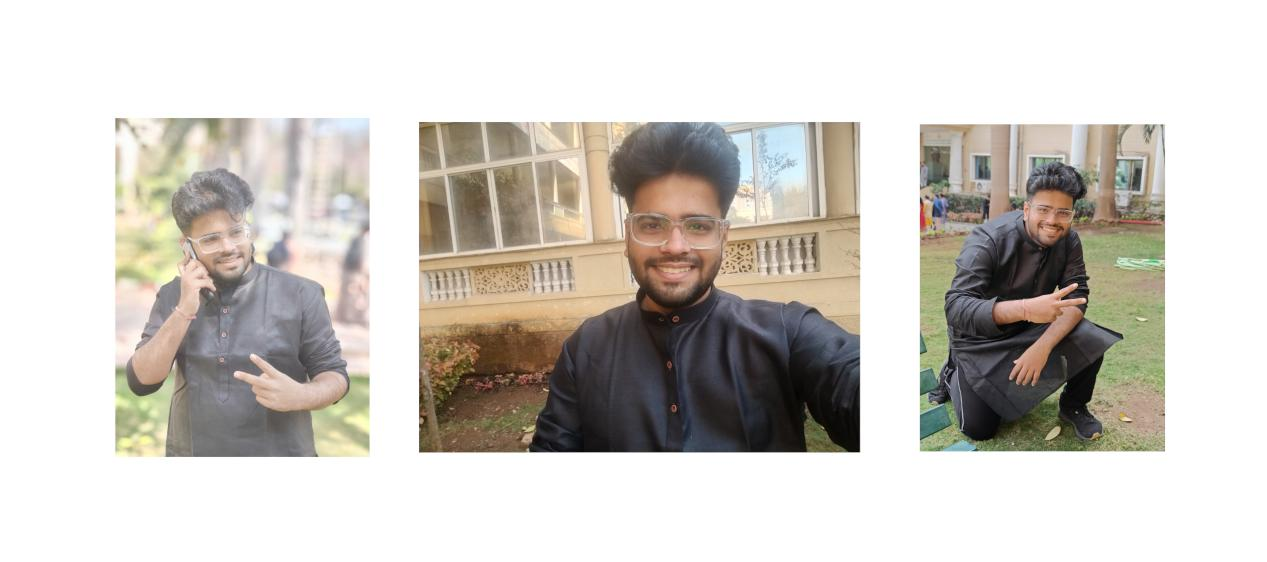
\includegraphics[width=.95\textwidth]{saubhagya.jpg}
			\caption{Images Uploaded under Saubhagya's Name, and PRN. }
		\end{figure}
	\end{minipage}
\end{frame}
\begin{frame}
	\centering
	\frametitle{Training Data}
	\framesubtitle{These Images were Uploaded using the API along with student details.}
	\begin{minipage}{0.95\textwidth}
		\begin{figure}[H]
			\centering
			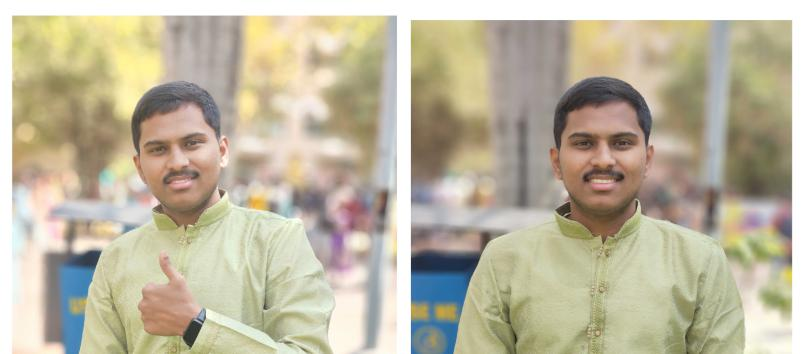
\includegraphics[width=.95\textwidth]{avishkar.jpg}
			\caption{Images Uploaded under Avishkar's Name, and PRN. }
		\end{figure}
	\end{minipage}
\end{frame}
\begin{frame}
	\centering
	\frametitle{Training Data}
	\framesubtitle{These Images were Uploaded using the API along with student details.}
	\begin{minipage}{0.95\textwidth}
		\begin{figure}[H]
			\centering
			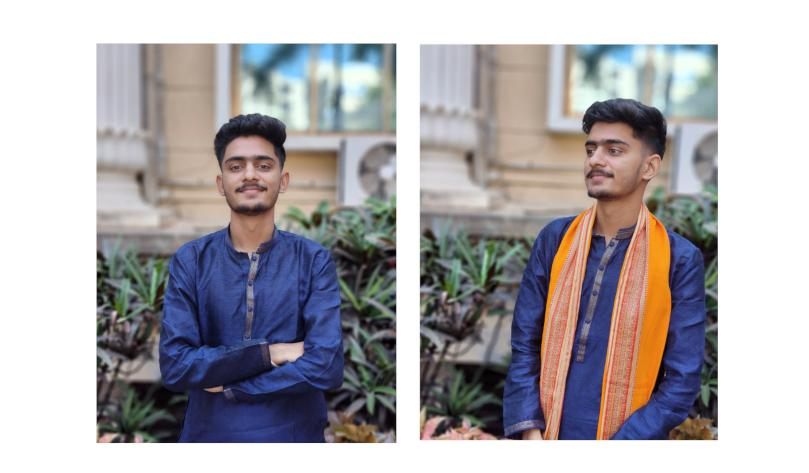
\includegraphics[width=.95\textwidth]{karad.jpg}
			\caption{}
		\end{figure}
	\end{minipage}
\end{frame}
\begin{frame}
	\centering
	\frametitle{Training Data}
	\framesubtitle{These Images were Uploaded using the API along with student details.}
	\begin{minipage}{0.95\textwidth}
		\begin{figure}[H]
			\centering
			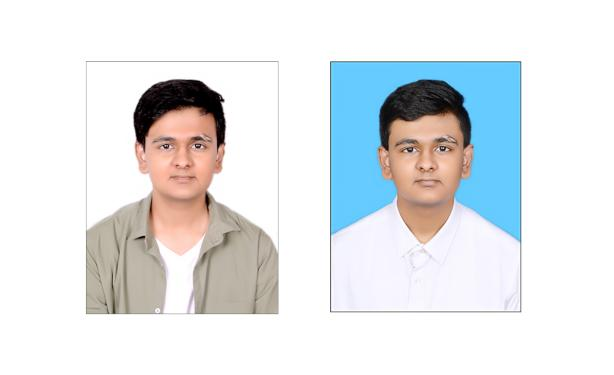
\includegraphics[width=.65\textwidth]{krish.jpg}
			\caption{These are the images uploaded under Krish's Name and PRN.}
		\end{figure}
	\end{minipage}
\end{frame}
\begin{frame}
	\centering
	\frametitle{Training Data}
	\framesubtitle{These Images were Uploaded using the API along with student details.}
	\begin{minipage}{0.95\textwidth}
		\begin{figure}[H]
			\centering
			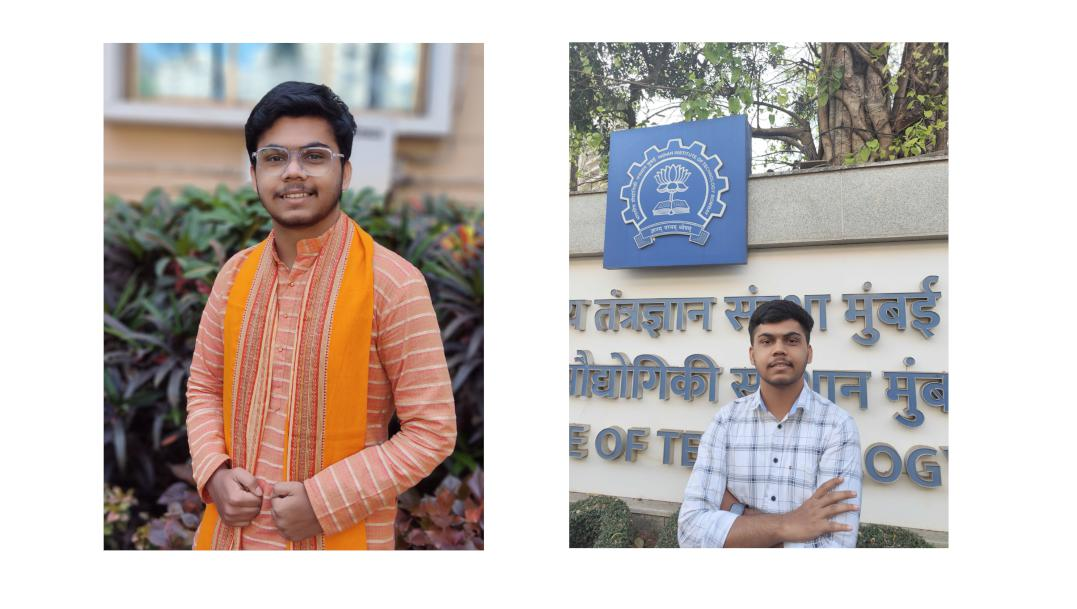
\includegraphics[width=.75\textwidth]{parth.jpg}
			\caption{These are the images uploaded under Parth's Name and PRN.}
		\end{figure}
	\end{minipage}
\end{frame}
\section{Preliminary Results}
\begin{frame}
	\centering
	\frametitle{Preliminary Results}
	\framesubtitle{Recognized Faces}
	\begin{minipage}{0.95\textwidth}
		\begin{figure}[H]
			\centering
			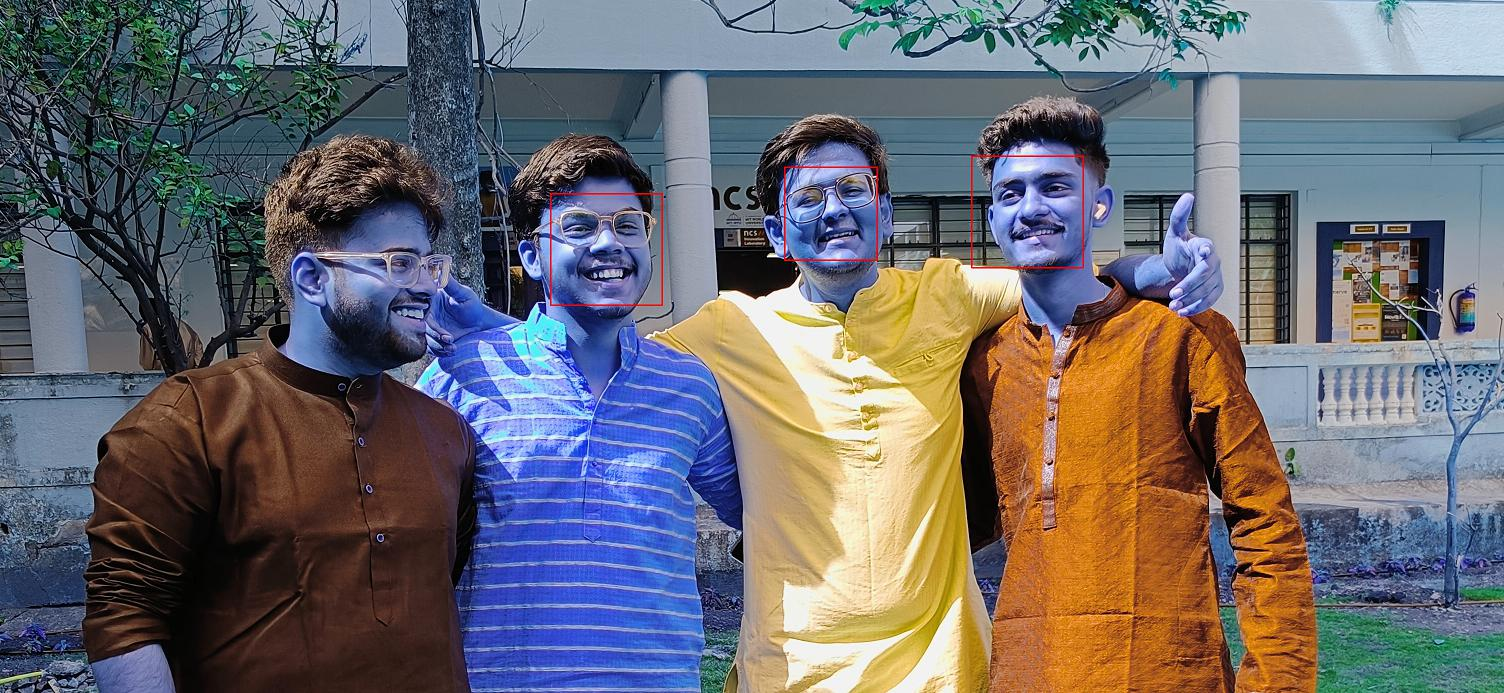
\includegraphics[width=.95\textwidth]{face rec results cropped.jpg}
			\caption{Results identifying 3 of the 4 faces. Empirical results show that the model is working, with accuracy of around 75 \%}
		\end{figure}	\end{minipage}
\end{frame}
\section{Backend Work Remaining}
\begin{frame}
	\centering
	\frametitle{Backend Work Remaining}
	\begin{minipage}{0.95\textwidth}
		\begin{enumerate}
			\item Complete the rest of the remaining APIs
			\item Test all APIs
			\item Integrate with Frontend
			\item Try out all the other libraries.
			\item Test with larger dataset
			\item Documentation of Results
		\end{enumerate}
	\end{minipage}
\end{frame}

\end{document}
